\section{Analysis of the per class OOD-generalization}
\label{section:real-separability}

In the previous section, performance on OOD detection methods in different representation spaces was analyzed using the overall AUROC measure. This is the standard metric in current literature for evaluating the performance of OOD detectors in OOD detection benchmarks.

This section proposes an essential extension of OOD evaluation to go beyond the overall AUROC measure in favor of per-class analysis –~i.e., presenting AUROC scores calculated per individual ID classes. This evaluation method allows the identification of the weak or worst-case ID classes, i.e., classes with low AUROC scores. This finding indicates a severe security gap in the deep model due to these classes, which realize low OOD generalization, i.e., are easily confused with OOD samples. In this way, the practitioners who implement AI models get additional insight into the safety risks of models deployed in safety-critical applications.

Because the research was performed per known in-distribution class, a~detailed illustration of the reached AUROC scores per representation and utilized outlierness measure can be created. Figure \ref{fig:image-auroc} presents the observed AUROC scores using bounding boxes for better understanding of the performance and measures/representation relations. The boxplots covers the median and upper/lower quarterly (50\% of observations), while the whiskers indicate the range of 95\% of results; the average values are marked with white dots for the reference. The key observations from this figure are:
\vspace{-0.5\baselineskip}
\begin{itemize}
    \item The performance of the outlierness measures is related to the utilized representation model. The detector that performed well for some representation, may be notably worse when used with feature vectors produced by other model – e.g., SED outperforms other measures for ResNet, while for ViT it turns to be the worst.
    \item In each case there exists significant number of classes that fall behind in terms of separability from outliers. Such classes can introduce security gaps in real-world applications of models and should be examined in safety-critical implementations.
    \item The models pre-trained on a large collection of image+text pairs (CLIP, CoCa) clearly outperformed other models in the task of separability. The ConvNeXT and ViT representations can also provide high-quality results, depending on the utilized outlierness measure. The ResNet turned out the worst in this task.
\end{itemize}

The results in figure \ref{fig:image-auroc} aggregate data for all classes from table \ref{tab:image-auroc}, while figure \ref{fig:image-auroc-detailed} contains the selected results per outlier data. No major differences can be observed between the analyzed dataset, indicating that the observed separability depends more on the utilized feature vectors representation and involved outlierness measure, rather than the examples that were examined.
This is test This is test This is test This is test This is test This is test

The results obtained for text documents are presented in figure \ref{fig:text-auroc-20newsgroups} and \ref{fig:text-auroc-banking77}. Similar conclusions can be drawn from the research – kNN perform best when used with BERT models, but falls out when used with fastText, where LOF offers the top-result, at the same time being the worst to use with BERT. In addition, it appears that the kind of utilized ID corpus plays the significant role as well – the separability (AUROC scores) was much better in case of short documents (sentences) rather than for longer documents (e-mails).

The lack of results for Mahalanobis distance (MD) in case of ConvNeXT and ResNet representation is a result of problems with covariance matrix estimation. Both representations utilize feature vectors of dimensions (section \ref{section:real-characteristics}, table \ref{tab:image-dimensions}) greater than the number of training samples available in the ImageNet dataset. The alternative suggested in literature in such cases is to utilize the Mahalanobis distance with pooled covariance matrix (MDP), however this approach turned out to be the worst possible overall in all analyzed cases.

\begin{figure}[t]
    % StreamLit settings: width=9, height=5
    \centering
    \vspace{-1.0em}  % spacing hack
    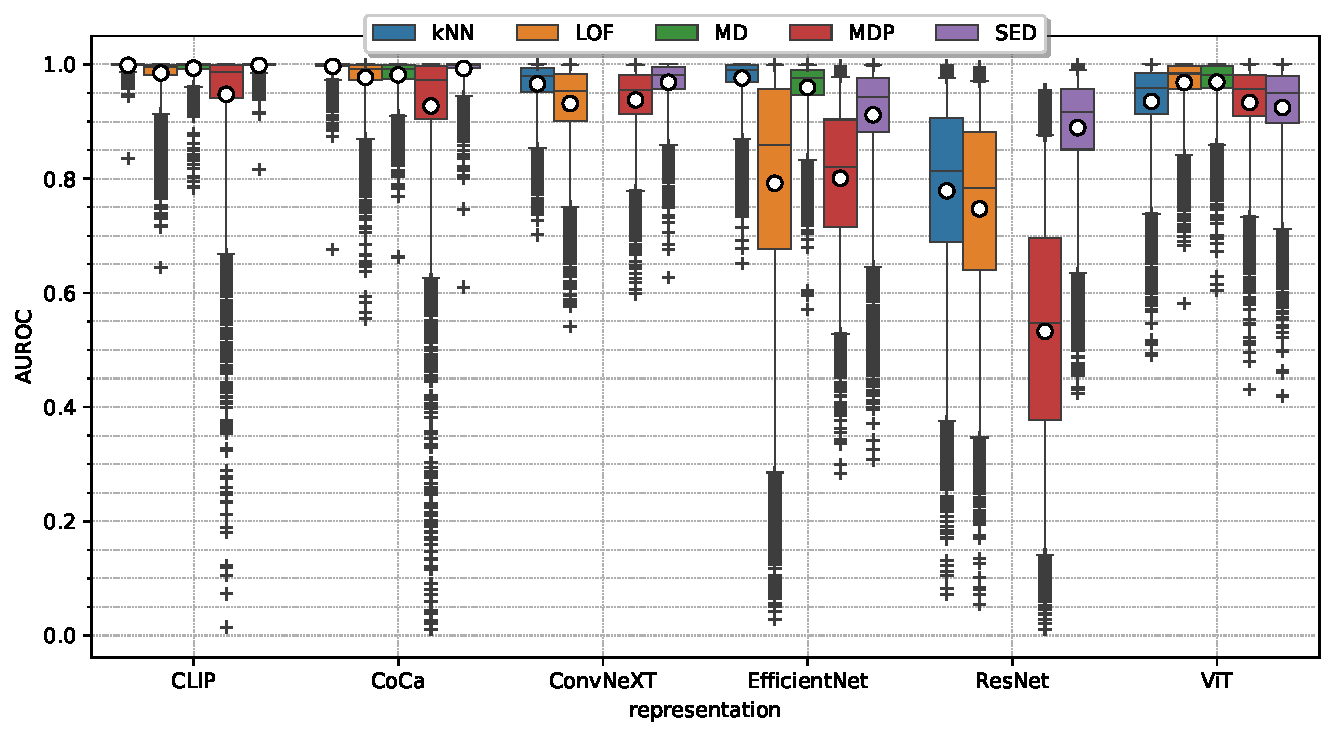
\includegraphics[width=\textwidth]{images/real-separability/barplot-ImageNet-auroc(representation,model)-representation_CLIP,CoCa,ConvNeXT,EfficientNet,ResNet,ViT-class_0,999-data_ALL.pdf}
    \caption{Observed separability between in-distribution data (ImageNet samples) and the out-of-distribution data from 7 datasets: ImageNet-O, iNaturalist, NINCO, OpenImage-O, Places365, SUN2012 and Textures. White dots mark the average scores, while the whiskers indicate the range of 95\% AUROC values calculated for a~given representation and outlierness measure. For some classes (marked with crosses) the~calculated AUROC value is very low, making them indistinguishable from outliers.}
    \label{fig:image-auroc}
    \vspace{-1.0em}  % spacing hack
\end{figure}

\begin{figure}[t]
    % StreamLit settings: width=9, height=4
    \centering
    \vspace{-0.5em}
    \begin{subfigure}[b]{0.9\textwidth}
        \centering
        \caption{\small Separability: ImageNet (ID) vs. ImageNet-O (OOD)}
        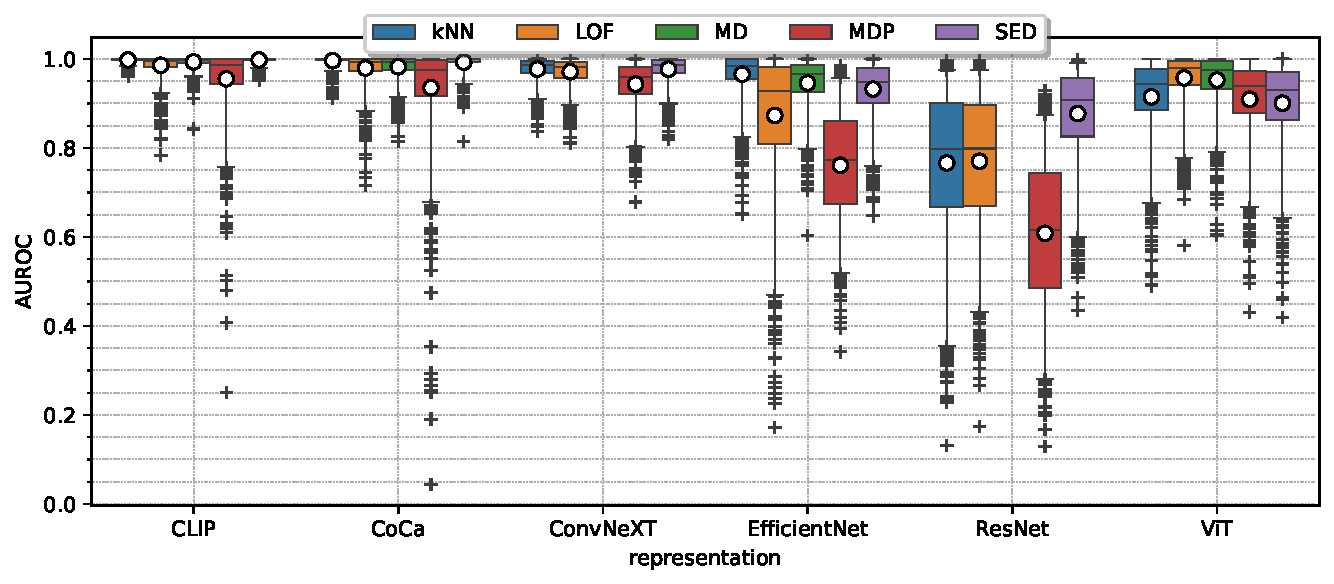
\includegraphics[width=\textwidth]{images/real-separability/barplot-ImageNet-auroc(representation,model)-representation_CLIP,CoCa,ConvNeXT,EfficientNet,ResNet,ViT-class_0,999-data_ImageNet-O.pdf}
        \label{fig:image-auroc-imagenet-o}
    \end{subfigure}

    \vspace{-0.5em}
    \begin{subfigure}[b]{0.9\textwidth}
        \centering
        \caption{\small Separability: ImageNet (ID) vs. Places365 (OOD)}
        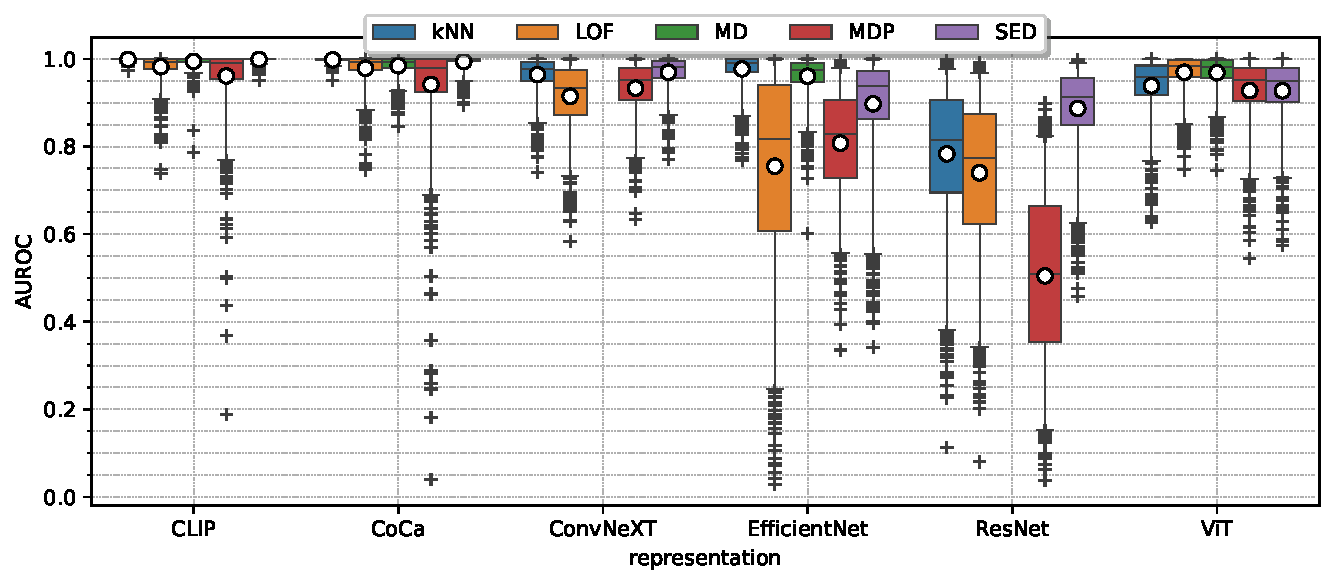
\includegraphics[width=\textwidth]{images/real-separability/barplot-ImageNet-auroc(representation,model)-representation_CLIP,CoCa,ConvNeXT,EfficientNet,ResNet,ViT-class_0,999-data_Places365.pdf}
        \label{fig:image-auroc-places365}
    \end{subfigure}

    \vspace{-0.5em}
    \begin{subfigure}[b]{0.9\textwidth}
        \centering
        \caption{\small Separability: ImageNet (ID) vs. SUN2012 (OOD)}
        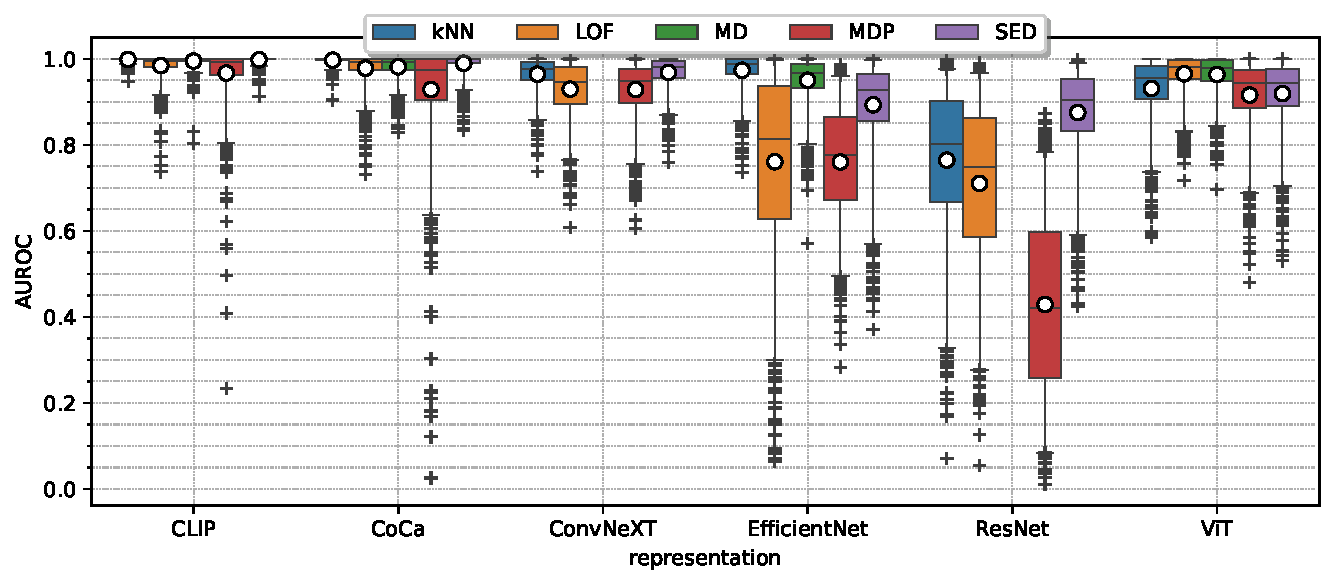
\includegraphics[width=\textwidth]{images/real-separability/barplot-ImageNet-auroc(representation,model)-representation_CLIP,CoCa,ConvNeXT,EfficientNet,ResNet,ViT-class_0,999-data_SUN2012.pdf}
        \label{fig:image-auroc-sun2012}
    \end{subfigure}
    \vspace{-0.5em}
    \caption{Detailed comparison of obtained AUROC scores per selected OOD data. No~major differences can be observed between the analyzed datasets, the utilized representation plays major role along with the chosen outlierness measure.}
    \label{fig:image-auroc-detailed}
\end{figure}

\begin{figure}[t]
    % StreamLit settings: width=9, height=5
    \centering
    \begin{subfigure}[b]{\textwidth}
        \centering
        \caption{\small Separability: 20newsgroups (17 ID classes vs. 3 OOD classes)}
        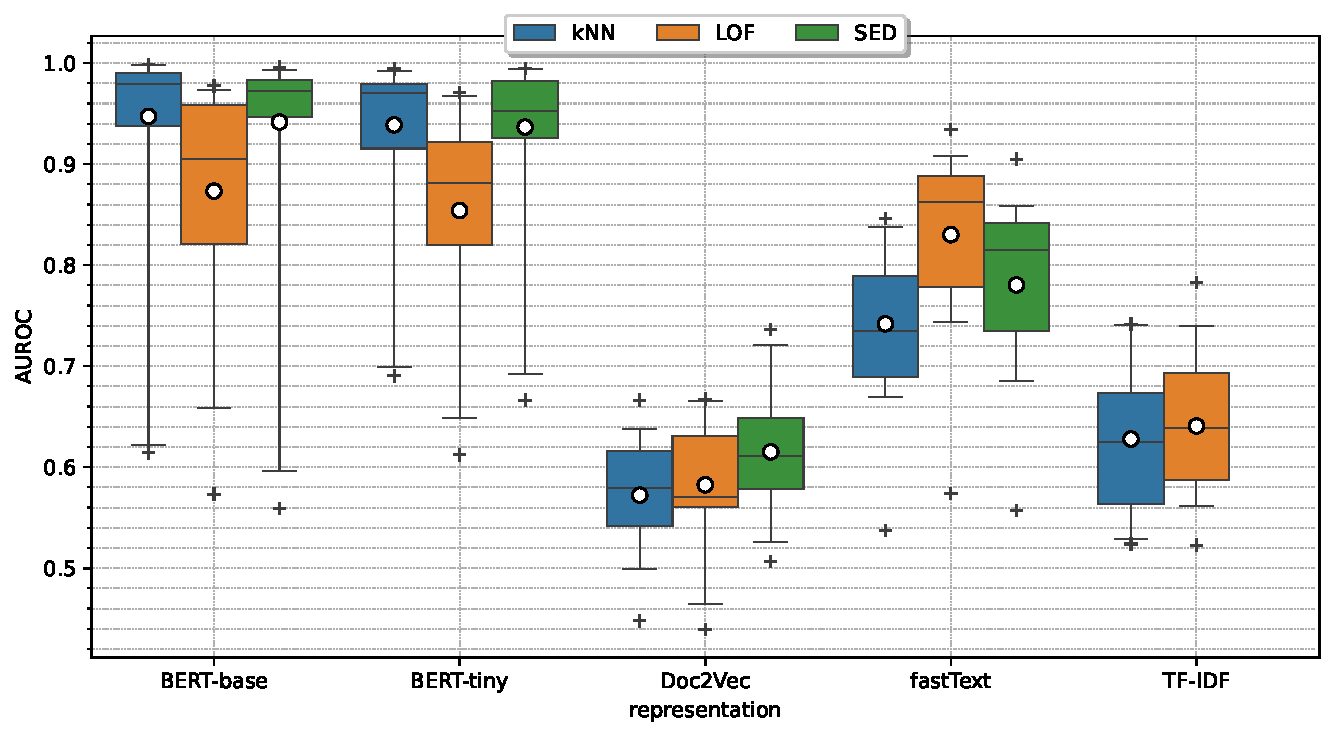
\includegraphics[width=\textwidth]{images/real-separability/barplot-20newsgroups-auroc(representation,model)-representation_BERT-base,BERT-tiny,Doc2Vec,fastText,TF-IDF-class_0,16-data_outlier.pdf}
        \label{fig:text-auroc-20newsgroups}
    \end{subfigure}
    \begin{subfigure}[b]{\textwidth}
        \centering
        \caption{\small Separability: banking77 (62 ID classes vs. 15 OOD classes)}
        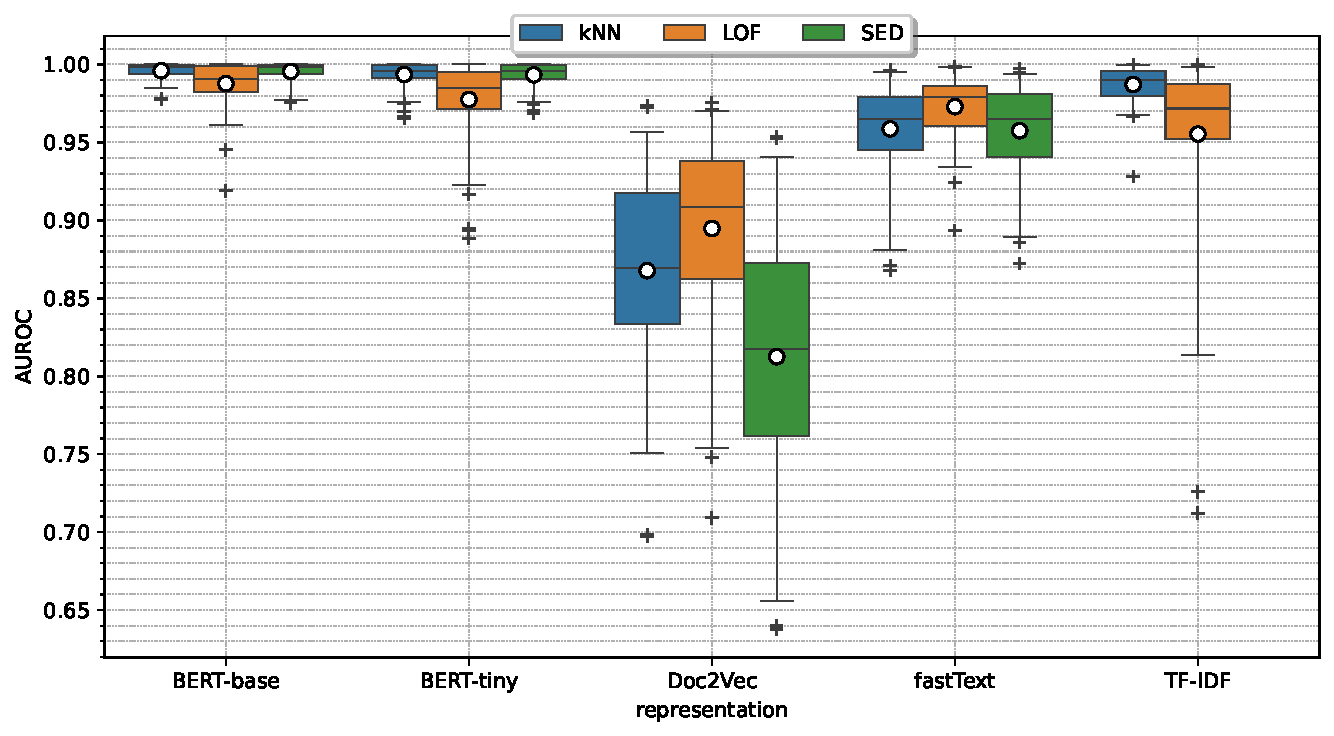
\includegraphics[width=\textwidth]{images/real-separability/barplot-banking77-auroc(representation,model)-representation_BERT-base,BERT-tiny,Doc2Vec,fastText,TF-IDF-class_0,61-data_outlier.pdf}
        \label{fig:text-auroc-banking77}
    \end{subfigure}
    \caption{Calculated AUROC scores, obtained in the separation task between the text data. In case of short documents (banking77) the separation task turns out to be much easier for all analyzed representations (all scores $\text{AUROC} \gtrsim 0.7$). The Doc2Vec and TF-IDF representations for 20newsgroups do not provide vectors suitable for performing the out-of-distribution detection.}
    \label{fig:text-auroc}
\end{figure}

\cleardoublepage{}
